\documentclass[28]{report}
\usepackage{graphicx} % Required for inserting images
\usepackage[a4paper, total={6in, 9in}]{geometry}
\usepackage{amsmath}
\usepackage{enumitem}
% \usepackage{minted}
\usepackage{float}
\usepackage{hyperref}
\hypersetup{
    colorlinks=true,
    linkcolor=black,
    filecolor=magenta,      
    urlcolor=cyan,
    pdftitle={Fast Fourier transform}
    }

\begin{document}

% \maketitle
\begin{titlepage}
    \centering
    \vspace*{2cm}
    
\includegraphics[width=0.25\textwidth]{images/buet.png}\\
    \vspace{1.5cm}
    {\Large \textbf{Bangladesh University of Engineering and Technology} \par}
    \vspace{2cm}
    {\LARGE \textbf{CSE 300} \par}
    \vspace{1cm}
    {\Large Report on \par}
    \vspace{0.5cm}
    {\LARGE \textbf{Fast Fourier Transform (FFT):\\[0.5em] A Revolutionizing Algorithm} \par}
    \vspace{1.5cm}
    {\large \textbf{Authors:} \par}
    \vspace{0.5cm}
    {\large Tanvirul Islam Turad (2005011) \par}
    {\large Tanvir Hossain (2005014) \par}
    {\large MD. Jakaria Hossain (2005026)\par}
    \vspace{2cm}
    {\large Date: \today \par}
\end{titlepage}

\tableofcontents
\newpage

\chapter{Introduction}
\section{Introduction}
The Fast Fourier Transform (FFT) is among the most important algorithms
in applied and engineering mathematics and in computer science because this algorithm allows us to multiply two polynomials of length 
$n$ in 
$O(n \log n)$ time, which is better than the trivial multiplication which takes 
$O(n^2)$ time.In the similar way two number of length $n$ can be multiplied by FFT in $O(n \log n)$ time. \linebreak 

In 1805, Karl Fredrich Gauss developed a method for fast calculation of Discrete Fourier Transform (DFT).\cite{wiki} But he never published it. Later on 1965, James Cooley and John Tukey published a very similar method. So, the credit of discovering the FFT is attributed to Cooley and Tukey. In fact the FFT has been discovered repeatedly before, but the importance of it was not understood before the inventions of modern computers. \\


Actually, the Fast Fourier Transform (FFT) is an algorithm to compute the Discrete Fourier Transform (DFT) and its inverse. It drastically reduces the computational complexity of computing
DFT, making it feasible for real-time processing.
% \pagebreak
\section{Motivation}
FFT is one of the top 10 algorithms of $20^{th}$ century included by the IEEE magazine {\it{Computing in Science and Engineering}}. FFT analyzes signals in the frequency domain to understand their
composition.\\ Limitations of the Discrete Fourier Transform (DFT):
 \begin{itemize}
        \item Quadratic time complexity, $O(N^2)$ \\ computationally expensive for large signals.
        \item Need for a faster and more efficient algorithm. FFT resolves in $O(n\log n)$.
      \end{itemize}
       FFT has taken revolution in the field of Signal processing (noise removal, filtering,...), Image processing (compression, feature extraction,...), Speech and audio processing (compression, synthesis,...), Scientific computing (solving differential equations, analyzing time-series data) etc.
% \pagebreak
\section{Fourier Transform}
Fourier Transform decomposes a signal into its frequency components.
It represents a signal in terms of sinusoidal basis functions.
\begin{itemize}
    \item The continuous Fourier Transform is given by:
    \[ F(\omega) = \int_{-\infty}^{\infty} f(t) e^{-i\omega t} dt \]
    where $f(t)$ is the signal, and $F(\omega)$ is its frequency domain representation.
  \end{itemize}

\section{Discrete Fourier Transform}

DFT is the discrete counterpart of the continuous Fourier Transform.
\begin{itemize}
    \item It is defined as:
    \[ X[k] = \sum_{n=0}^{N-1} x[n] e^{-i2\pi kn/N} \]
    where $x[n]$ is the discrete signal, and $X[k]$ is its frequency domain representation.
      \end{itemize}
Direct computation of DFT is of $O(N^2)$ complexity.\cite{cp_algo}
% \pagebreak
\subsection{Polynomial Representation}
To understand the use of Discrete Fourier Transform let's take an example of a polynomial. The polynomial is of $(n-1)^{th}$ order where $n$ can be either power of 2 or not. If it is not a power of 2 then take some extra terms of higher order putting the coefficients of those terms $p_i$ 0. \\
              \begin{equation*}
                  P(x) = p_0 + p_1x + p_2x^2 + ... + p_{n-1}x^{n-1}
              \end{equation*}
              From complex number we know that the equation $z^n = 1$ has $n$ complex solutions (called the $n$-th roots of unity), and the solutions are of the form $w_{k} = e^{\frac{2 k \pi i}{n}}$ with $k = 0 \dots n-1$. Additionally these complex numbers have some very interesting properties: e.g. the principal $n$-th root $ w_{1} = e^{\frac{2 \pi i}{n}}$ can be used to describe all other $n$-th roots: $w_{k} = w^k$.
              \\
              
              The following figure best describes the senario:

               \begin{figure}[H]
               \centering
               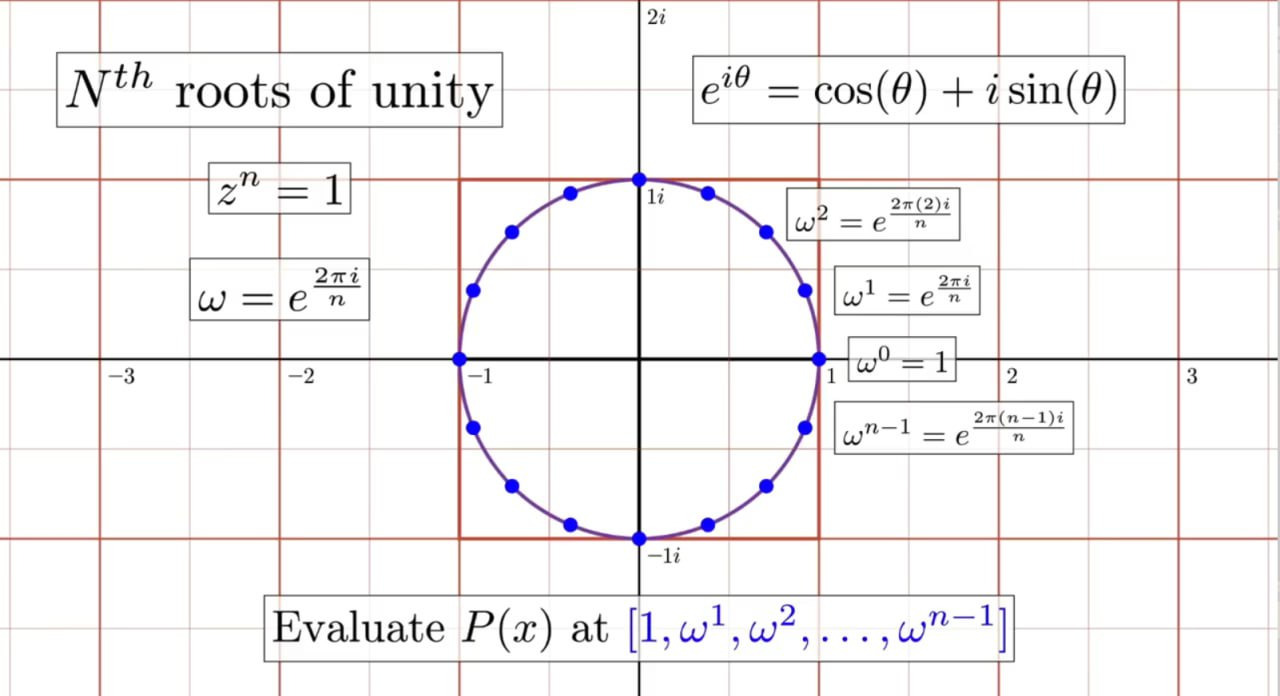
\includegraphics[width=1\textwidth]{images/nthroot.jpg}
               
               \label{fig:enter-label}
               \end{figure}

              The polynomial $P(x)$ can equivalently be represented as the vector of coefficients $(p_0, p_1, \dots, p_{n-1})$. The Discrete Fourier Transform of the polynomial is defined as the values of the polynomial at the points $x = w_{k}$, i.e. it is the vector: \\

                \begin{align*} \text{DFT}(p_0, p_1, \dots, p_{n-1}) &= (y_0, y_1, \dots, y_{n-1}) \\ &= (P(w_{0}), P(w_{1}), \dots, P(w_{n-1})) \\ &= (P(w^0), P(w^1), \dots, P(w^{n-1})) \end{align*}
                % \pagebreak

            On the other hand,  the Inverse Discrete Fourier Transform is defined: The inverse DFT of values of the polynomial $(y_0, y_1, \dots, y_{n-1})$ are the coefficients of the polynomial $(p_0, p_1, \dots, p_{n-1})$.
            $$\text{InverseDFT}(y_0, y_1, \dots, y_{n-1}) = (p_0, p_1, \dots, p_{n-1})$$

            Thus by using the $n^{th}$ roots of unity we can find the DFT of a polynomial( DFT on coefficients ) and by the Inverse DFT (Inverse DFT on values ) we again can restore the original coefficients of the polynomial.
            \\
            
            For fast multiplication of two polynomials DFT and Inverse DFT can be used. First find the DFT of the two polynomials let say ( $M(x)$ and $N(x)$ ) and their DFTs are $ DFT(M)$ and $ DFT(N) $.\\
            

             If we multiply the vectors $\text{DFT}(M)$ and $\text{DFT}(N)$ - by multiplying each element of one vector by the corresponding element of the other vector - then we get nothing other than the DFT of the polynomial $\text{DFT}(M \cdot N)$:
            $$\text{DFT}(M \cdot N) = \text{DFT}(M) \cdot \text{DFT}(N)$$

            Here, on the right side multiplication of DFTs we mean the pairwise product of the vector elements. This can be computed in $O(n)$ time. Next we do Inverse DFT on the result\\
            $$M \cdot N = \text{InverseDFT}(\text{DFT}(M) \cdot \text{DFT}(N))$$

            If this calculation needs $O(n\log n)$ computational steps, then the overall time complexity of the algorithm will be $O(n\log n)$.
            
\section{Fast Fourier Transform}

Fast Fourier Transform(FFT) is the solution of the previous computational complexity problem. Applying FFT the complexity can be reduced to $O(n\log n)$.Basically this algorithm uses divide and conquer technique to resolve the issue.\\

Let's take a polynomial $P(x)$ of order is $n-1$, where $n$ is a power of 2.

 $$P(x) = p_0 + p_1x 
 + p_2x^2 + ... + p_{n-1}x^{n-1}$$\\
 
 We divide it into two smaller polynomials, the one containing only the coefficients of the even positions, and the one containing the coefficients of the odd positions:
  \begin{align*} P_o(x) &= p_0 x^0 + p_2 x^1 + \dots + p_{n-2} x^{\frac{n}{2}-1} \\ P_e(x) &= p_1 x^0 + p_3 x^1 + \dots + p_{n-1} x^{\frac{n}{2}-1} \end{align*}

  % \pagebreak
  The polynomial can also be represented as:\\
  $$P(x) = P_o(x^2) + x P_e(x^2).$$

  
The polynomials $P_o$ and $P_e$ are only half as much coefficients as the polynomial $P$. If we can compute the $\text{DFT}(P)$ in linear time using $\text{DFT}(P_o)$ and $\text{DFT}(P_e)$, then we get the recurrence $T_{\text{DFT}}(n) = 2 T_{\text{DFT}}\left(\frac{n}{2}\right) + O(n)$ for the time complexity, which results in $T_{\text{DFT}}(n) = O(n \log n)$ by the master theorem.\\

Let's say we have already computed the $\left(y_k^o\right)_{k=0}^{n/2-1}$ = $DFT(P_o)$ and \\ $\left(y_k^e\right)_{k=0}^{n/2-1}$ =$DFT(P_e)$\\ 

For the first $\frac{n}{2}$ values we can just use the previously noted equation\\ $P(x) = P_o(x^2) + x P_e(x^2)$:
$$y_k = y_k^o + w^k y_k^e, \quad k = 0,1, \dots ,\frac{n}{2} - 1.$$

The next $\frac{n}{2}$ values we need to find an expression which is pretty similar to our last expression of finding first half:
\begin{align*} y_{k+n/2} &= P\left(w^{k+n/2}\right) \\ &= P_o\left(w^{2k+n}\right) + w^{k + n/2} P_e\left(w^{2k+n}\right) \\ &= P_o\left(w^{2k} w^n\right) + w^k w^{n/2} P_e\left(w^{2k} w^n\right) \\ &= P_o\left(w^{2k}\right) - w^k P_e\left(w^{2k}\right) \\ &= y_k^o - w^k y_k^e \end{align*}






Here we used again $P(x) = P_o(x^2) + x P_e(x^2)$ and the two identities $w^n = 1$ and $w^{n/2} = -1$.

Therefore we get the desired formulas for computing the whole vector $(y_k)$:
\begin{align*} y_k &= y_k^o + w^k y_k^e, &\quad k = 0 \dots \frac{n}{2} - 1, \\ y_{k+n/2} &= y_k^o - w^k y_k^e, &\quad k = 0 \dots \frac{n}{2} - 1. \end{align*}

Thus we learned how to compute the DFT in $O(n \log n)$ time.\\
To know more check this\cite{fftbook1} book.

\chapter{Applications}
FFT is the core component of frequency domain analysis, also known as spectrum analysis, in signal processing. It is widely used in data compression, spectral estimation, signal filtering, and other applications. Analysis in both the frequency and time domains can be done simultaneously using FFT variations like the short-time Fourier transform. These methods can be applied to a wide range of signals, including communication, radar, audio and speech, and other sensor data signals. Additionally, FFT is occasionally employed as a transitional step before more sophisticated signal processing methods. FFT is used for filtering and picture compression in image processing. In mathematics and physics, partial differential equations (PDEs) are also solved using FFT.
\section{FFT in signal processing}
FFT is most frequently used to convert signals from the time domain to the frequency domain.
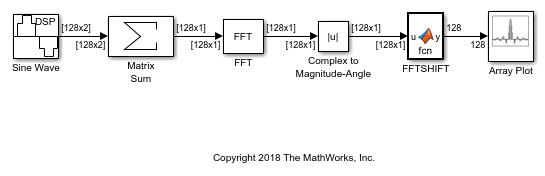
\includegraphics[scale=0.8]{images/t_f_dom.png}
The fundamental algorithm used for time-frequency based signal analysis in many simulation programs, such as MATLAB, is FFT. The FFT algorithm was utilized by MATLAB's\cite{matlab} Signal Processing $Toolbox^{TM}$ to display spectograms and persistent spectrums, which are time-frequency views that display the proportion of a signal's duration that a certain frequency is present.\\
\begin{tabular}{c c}
    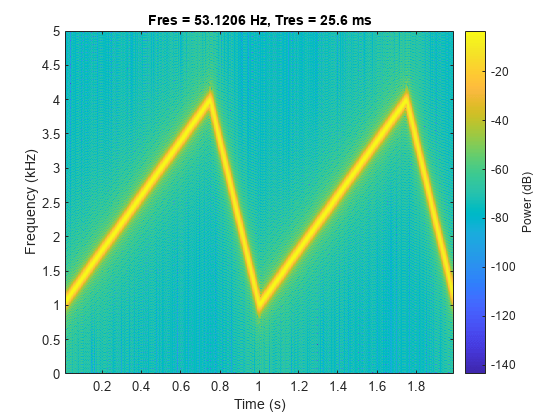
\includegraphics[scale=0.35]{images/signal_1.png}    &  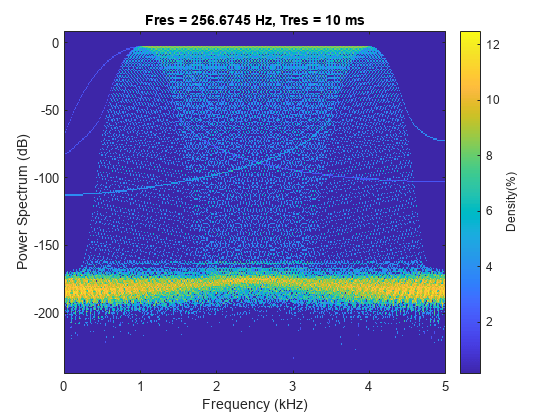
\includegraphics[scale=0.35]{images/signal_2.png}
\end{tabular}
FFT helps in radar signal analysis, target detection, and tracking. FFT aids in underwater acoustics, target detection, and classification. 
\section{FFT in Communications}
    \begin{itemize}[]
            \item Digital communication systems: FFT is utilized in modulation and demodulation schemes such as OFDM (Orthogonal Frequency Division Multiplexing) used in Wi-Fi, LTE, and digital television.
            \item Channel estimation and equalization: FFT helps in estimating the channel characteristics and compensating for distortions in communication channels.
    \end{itemize}
\section{FFT in Instrumentation}
\begin{itemize}[]
            \item Spectrum analysis: FFT is employed in spectrum analyzers for measuring frequency components of signals.
            \item Biomedical signal analysis: FFT is used in the analysis of EEG (Electroencephalography), ECG (Electrocardiography), and other biomedical signals for diagnosis and monitoring.
        \end{itemize}
\section{FFT in Control Systems}
    \begin{itemize}[]
            \item Control system analysis: FFT is used in identifying system dynamics, frequency response analysis, and stability analysis.
            \item Control system design: FFT helps in designing controllers and compensators for systems with frequency-dependent characteristics.
    \end{itemize}
\section{FFT in Geophysics and Seismology}
    \begin{itemize}[]
        \item Earthquake analysis: FFT is used in seismic data processing for earthquake detection, location, and magnitude estimation.\\
        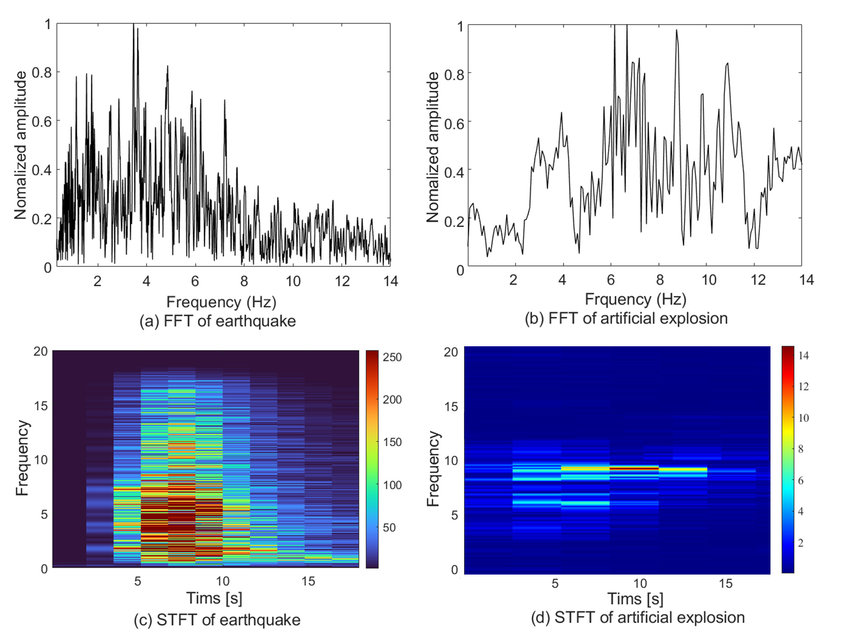
\includegraphics[scale=0.5]{images/seismic_signal_1.jpg}
        \item Exploration geophysics: FFT assists in the interpretation of seismic data for oil and gas exploration.
    \end{itemize}
\section{FFT in Medical Imaging}
    \begin{itemize}[]
        \item MRI (Magnetic Resonance Imaging): FFT is utilized in MRI for image reconstruction from raw data acquired during scans.
        \item CT (Computed Tomography): FFT is used in image reconstruction algorithms to convert raw projection data into cross-sectional images.
    \end{itemize}
\section{FFT in Astrophysics and Cosmology}
    \begin{itemize}[]
        \item Radio astronomy: FFT is employed in processing radio signals received from celestial objects for analysis and imaging.
        \item Cosmology: FFT assists in analyzing cosmic microwave background radiation data for studying the early universe.
    \end{itemize}
\section{FFT in Computer Science}
DFT, a special variation of FFT can be used in a huge variety of other problems, which at the first glance have nothing to do with multiplying polynomials.

\subsection{All possible sums}

We are given two arrays $a[]$ and $b[]$. We have to find all possible sums $a[i] + b[j]$, and for each sum count how often it appears.

For example for $a = [1,~ 2,~ 3]$ and $b = [2,~ 4]$ we get: then sum $3$ can be obtained in $1$ way, the sum $4$ also in $1$ way, $5$ in $2$, $6$ in $1$, $7$ in $1$.

We construct for the arrays $a$ and $b$ two polynomials $A$ and $B$. The numbers of the array will act as the exponents in the polynomial ($a[i] \Rightarrow x^{a[i]}$); and the coefficients of this term will be how often the number appears in the array.

Then, by multiplying these two polynomials in $O(n \log n)$ time, we get a polynomial $C$, where the exponents will tell us which sums can be obtained, and the coefficients tell us how often. To demonstrate this on the example:
$$(1 x^1 + 1 x^2 + 1 x^3) (1 x^2 + 1 x^4) = 1 x^3 + 1 x^4 + 2 x^5 + 1 x^6 + 1 x^7$$

\subsection{All possible scalar products}

We are given two arrays $a[]$ and $b[]$ of length $n$. We have to compute the products of $a$ with every cyclic shift of $b$.

We generate two new arrays of size $2n$: We reverse $a$ and append $n$ zeros to it. And we just append $b$ to itself. When we multiply these two arrays as polynomials, and look at the coefficients $c[n-1],~ c[n],~ \dots,~ c[2n-2]$ of the product $c$, we get:
$$c[k] = \sum_{i+j=k} a[i] b[j]$$

And since all the elements $a[i] = 0$ for $i \ge n$:
$$c[k] = \sum_{i=0}^{n-1} a[i] b[k-i]$$

It is easy to see that this sum is just the scalar product of the vector $a$ with the $(k - (n - 1))$-th cyclic left shift of $b$. Thus these coefficients are the answer to the problem, and we were still able to obtain it in $O(n \log n)$ time. Note here that $c[2n-1]$ also gives us the $n$-th cyclic shift but that is the same as the $0$-th cyclic shift so we don't need to consider that separately into our answer.

\subsection{Two stripes}

We are given two Boolean stripes (cyclic arrays of values $0$ and $1$) $a$ and $b$. We want to find all ways to attach the first stripe to the second one, such that at no position we have a $1$ of the first stripe next to a $1$ of the second stripe.

The problem doesn't actually differ much from the previous problem. Attaching two stripes just means that we perform a cyclic shift on the second array, and we can attach the two stripes, if scalar product of the two arrays is $0$.

\subsection{String matching}

We are given two strings, a text $T$ and a pattern $P$, consisting of lowercase letters. We have to compute all the occurrences of the pattern in the text.

We create a polynomial for each string ($T[i]$ and $P[I]$ are numbers between $0$ and $25$ corresponding to the $26$ letters of the alphabet):
$$A(x) = a_0 x^0 + a_1 x^1 + \dots + a_{n-1} x^{n-1}, \quad n = |T|$$

with
$$a_i = \cos(\alpha_i) + i \sin(\alpha_i), \quad \alpha_i = \frac{2 \pi T[i]}{26}.$$

And
$$B(x) = b_0 x^0 + b_1 x^1 + \dots + b_{m-1} x^{m-1}, \quad m = |P|$$

with
$$b_i = \cos(\beta_i) - i \sin(\beta_i), \quad \beta_i = \frac{2 \pi P[m-i-1]}{26}.$$

Notice that with the expression $P[m-i-1]$ explicitly reverses the pattern.

The $(m-1+i)$th coefficients of the product of the two polynomials $C(x) = A(x) \cdot B(x)$ will tell us, if the pattern appears in the text at position $i$.
$$c_{m-1+i} = \sum_{j = 0}^{m-1} a_{i+j} \cdot b_{m-1-j} = \sum_{j=0}^{m-1} \left(\cos(\alpha_{i+j}) + i \sin(\alpha_{i+j})\right) \cdot \left(\cos(\beta_j) - i \sin(\beta_j)\right)$$

with $\alpha_{i+j} = \frac{2 \pi T[i+j]}{26}$ and $\beta_j = \frac{2 \pi P[j]}{26}$

If there is a match, than $T[i+j] = P[j]$, and therefore $\alpha_{i+j} = \beta_j$. This gives (using the Pythagorean trigonometric identity):
\begin{equation*}
    \begin{align*}
     c_{m-1+i} &= \sum_{j = 0}^{m-1} \left(\cos(\alpha_{i+j}) + i \sin(\alpha_{i+j})\right) \cdot \left(\cos(\alpha_{i+j}) - i \sin(\alpha_{i+j})\right) \\
     &= \sum_{j = 0}^{m-1} \cos(\alpha_{i+j})^2 + \sin(\alpha_{i+j})^2 = \sum_{j = 0}^{m-1} 1 = m 
    \end{align*}
\end{equation*}

If there isn't a match, then at least a character is different, which leads that one of the products $a_{i+1} \cdot b_{m-1-j}$ is not equal to $1$, which leads to the coefficient $c_{m-1+i} \ne m$.

\subsection{String matching with wildcards}

This is an extension of the previous problem. This time we allow that the pattern contains the wildcard character $\*$, which can match every possible letter. E.g. the pattern $a*c$ appears in the text $abccaacc$ at exactly three positions, at index $0$, index $4$ and index $5$.

We create the exact same polynomials, except that we set $b_i = 0$ if $P[m-i-1] = *$. If $x$ is the number of wildcards in $P$, then we will have a match of $P$ in $T$ at index $i$ if $c_{m-1+i} = m - x$.

% \newpage

\subsection*{More problems to explore\cite{cf_1} \cite{cc_1}}

\begin{itemize}

\item \href{https://www.spoj.com/problems/POLYMUL/}{POLYMUL - Polynomial Multiplication}

\item \href{https://www.spoj.com/problems/MAXMATCH/}{MAXMATCH - Maximum Self-Matching}

\item \href{https://www.spoj.com/problems/ADAMATCH/}{ADAMATCH - Ada and Nucleobase}

\item \href{https://codeforces.com/problemset/problem/954/I}{Yet Another String Matching Problem\cite{cf_2}}

\item \href{https://codeforces.com/problemset/problem/958/F3}{Lightsabers (hard)\cite{cf_3}}

\item \href{https://codeforces.com/contest/1398/problem/G}{Running Competition\cite{cf_4}}

\item \href{https://codeforces.com/contest/754/problem/E}{Dasha and cyclic table\cite{cf_5}}

\item \href{https://codeforces.com/problemset/problem/1667/E}{Centroid Probabilities\cite{cf_6}}

\item \href{https://www.codechef.com/COOK112A/problems/MMNN01}{Expected Number of Customer}

\item \href{https://www.codechef.com/SEPT19A/problems/PSUM}{Power Sum}

\item \href{https://open.kattis.com/problems/aplusb}{A+B Problem}

\item \href{https://open.kattis.com/problems/kinversions}{K-Inversions}

\end{itemize}
\chapter{Conclusion}

In conclusion, the Fast Fourier Transform (FFT) technique is a cornerstone in signal processing and beyond. Its extraordinary efficiency in computing the Discrete Fourier Transform (DFT) has enabled advances in a wide range of applications.

Throughout this report, we have explored the diverse applications of the FFT algorithm, spanning signal processing, communications, instrumentation, control systems, geophysics, medical imaging, finance, astrophysics, and cosmology. From audio and image processing to radar and sonar signal analysis, from medical diagnostics to seismic data interpretation, the FFT algorithm finds itself at the heart of countless innovative solutions.

The versatility of the FFT algorithm supports vital technologies like digital communication networks, medical imaging equipment, and astronomical observatories in addition to making signal analysis and modification easier. Its widespread use highlights its significance as a vital instrument in contemporary research and engineering.

Looking ahead, as technology continues to evolve, the FFT algorithm is poised to remain an indispensable asset, enabling further breakthroughs in fields ranging from data science to space exploration. Its impact on our understanding of the world and our ability to manipulate and interpret signals is undeniable, making it a subject of continued research and application for years to come.

In essence, the FFT algorithm exemplifies the power of computational methods to unlock new insights and capabilities across a broad spectrum of disciplines, shaping the landscape of scientific inquiry and technological innovation.
\newpage
\renewcommand{\bibname}{References}
\bibliographystyle{plain}
\bibliography{ref}
\end{document}